\chapter*{\FontH{\Huge Der kleine Pirat Winnimon}}
\addcontentsline{toc}{chapter}{Der kleine Pirat Winnimon}
\section*{\center $\skull$ Die Prüfung $\skull$}
\lettrine[lines=3]{\color{red}W}{ie} jeder andere Pirat auch, war Winniemon nicht schon immer ein Pirat. Genau wie du und ich war er zunächst ein kleiner Junge, der höchstens einmal mit dem Boot seines Opas zum Angeln auf dem Meer gewesen ist. 

\todo{Aye. Dorf der Waisen. Piratengesetze-Mitspracherecht, Spanier, Klabautermann, Jolly Roger, Krähennest, Kombüse, Smutje, Papagei, Seemannsknoten, Bukanier}
Aber auch das war er nicht besonders oft, denn Winnimon hatte ein Problem, für das er sich sehr geschämt hat. Er konnte nicht schwimmen! Piraten müssen aber schwimmen können, das ist klar. Piraten müssen nämlich ständig Mutproben machen, da kann es schon einmal vorkommen, dass man mit verbundenen Augen und einem Messer im Mund auf der Reeling balancieren muss. Und wenn man dann den kleinsten Fehler macht, liegt man im Meer.

Wenn man nicht schwimmen kann, sollte man sich lieber einen anderen Beruf aussuchen. Das kam für Winnimon aber nicht in Frage. Undenkbar! Der Vater war ein Pirat und sein grosser Bruder war auch einer. Und was viel wichtiger war: alle seine Freunde wollten Pirat werden. Und die konnten schwimmen, die brauchten sich keine Sorgen zu machen.

Wenn man auf einem Piratenschiff anheuern möchte, muss man drei Prüfungen bestehen. Erstens muss man fluchen können wie ein alter Papagei. Das klappte bei Winnimon ausgezeichnet, jedenfalls fand das seine Mutter, die aber allgemein nicht viel für Flüche übrig hatte. 

\enquote{Du dreifach stinkender Pups einer blinden Robbe} war Winnimons Lieblingsfluch. Den hatte er erst einmal gesagt, als grosser Bruder ihm einmal zum Frühstück eine leere Eischale hingesetzt hatte. Die Mutter hätte ihm fast eine Ohrfeige gegeben, was aber ein gutes Zeichen war. Denn seitdem wusste er, welchen Fluch er zur ersten Piratenprüfung fluchen würde. Den hatte er lieber nicht noch einmal geflucht, nicht dass ihm den noch jemand von seinen Freunden klaut!

Die zweite Prüfung war auch nicht so schwer. Man musste lesen und schreiben können. Erstens musste man der Mutter eine Flaschenpost schicken können, falls zum Beispiel die Socken so alt waren, dass sie neue schicken musste oder wenn man einfach Heimweh hatte. Das darf man sogar als Pirat haben, der gerade durch ferne Meere kreuzt. Und man musste natürlich Schatzkarten lesen können. Wenn da steht \enquote{Der Schatz liegt auf der Insel Woladimadudistan} ist das schon besser, sonst muss man den Schatz auf allen Inseln suchen und von denen gibt es viele. Aber Winnimon war zwar nicht so schlau wie die lange Druda aus seiner Klasse, aber Lesen und Schreiben klappten prima. Kein Problem also, die zweite Piratenprüfung.

Es blieb nur die Sache mit dem Schwimmen. Nicht dass Winnimon es nicht immer wieder einmal probieren würde. Aber er zappelte nur, der grosse Bruder lachte, der Vater war ärgerlich und nach dem zweiten Schluck Wasser, dass er unfreiwillig getrunken hatte, gab er immer auf. Wie machten das die anderen bloss? Wen er probierte, nicht mehr mit den Beinen auf dem Boden zu stehen, ging der Kopf automatisch unter Wasser. Schrecklich! Er hatte gar keine Zeit, überhaupt nur einmal einen Schwimmzug zu probieren.

In dem kleinen Dorf, in dem er wohnte, herrschte grosse Aufregung. Ein Piratenschiff hatte sich angekündigt, in drei Wochen schon sollte es da sein. Es wurden Jungen gesucht, die mit auf See wollten. Und Winnimon wollte. Und wie er wollte! Pirat sein, das ist das Grösste! Sofort machte er sich auf zum Meer, schwimmen üben. Noch drei Wochen, bis dahin musste das klappen, unbedingt. 

Am Strand waren schon die anderen Jungen versammelt, auch die, die nicht Pirat werden wollten. Sie hatten aus Brettern ein Floss gebastelt und spielten natürlich Pirat. Sie sprangen von Floss ins Wasser und schwammen um die Wette. Winnimon zog seine Badehose und watete vorsichtig ein paar Schritte ins Meer. Die Wellen schwapptem ihm gegen den Bauch. Er wusste nicht einmal, wie er anfangen sollte zu üben. Er wartete auf ein Tal zwischen zwei Wellen und kniete sich hin. Aber schon spülte die nächste Welle ihn im hohen Bogen ans Ufer zurück. 

Den anderen war das traurige Schauspiel natürlich nicht entgangen. Lachend und schreiend kamen sie angerannt und hänselten Winnimon.

\enquote{Seht Euch mal den an, der Schwimmt ein Sack voller Steine!} war noch das Harmloseste. Obwohl Piraten nie weinen, kullerten Winnimon ein paar Tränen über die Wangen. Nicht weil die anderen ihn gehänselt haben, das war nicht so schlimm, so was kommt vor, er hat ja auch schon mitgemacht. Das Schlimme war, dass sie ja Recht hatten. Er schwamm tatsächlich genau so wie ein Sack voller Steine: immer direkt nach unten.

Eine Hand legte sich auf seine Schulter. Die lange Druda stand hinter ihm. An jedem anderen Tag wäre Winnimon vor Scham im Erdboden versunken, wenn ein Mädchen ihn weinen sieht, aber heute war ihm alles egal. Schluchzend erklärte er ihr, warum er so weinen musste. Druda überlegte. 

\enquote{Also pass auf} sagte sie. \enquote{Ich bringe dir das Schwimmen bei. Aber Du musst dann auch etwas für mich tun. Versprichst Du das?}

Winnimon zögerte keinen Augenblick. \enquote{Alles, was Du willst!}

\enquote{Na gut, dann komm morgen früh zum Waldrand. Und bring zwei Rumfässer und ein Seil mit.}

Ausgerüstet mit den verlangten Dingen und einer frisch gewaschenen Badehose stand Winnimon schon am Waldrand, bevor es hell wurde. Druda kam pünktlich zum Sonnenaufgang und hatte nicht vergessen, etwas zum Essen mitzubringen. Als erstes sträkten sich die beiden, dann gingen sie zu dem kleinen Waldsee, der ein bisschen versteckt war.

\todo{Zeitformen anpassen}
\enquote{Hier wirst du schwimmen lernen} sagt sie. \enquote{Das Wasser hier ist ruhig, da kann man besser üben. So, und jetzt binden wir den Strick zwischen die beiden Fässer, aber so, dass noch etwas Platz dazwischen ist.}

Knoten konnte Winnimon schon sehr gut und so dauerte es nicht lange, bis er fertig war. Die Fässer sollten als Schwimmer dienen, er selbst legte sich auf die Seile dazwischen. So konnte er nicht untergehen. Druda zeigt ihm mit viel Geduld wie man schwimmt. Die Beine wie ein Frosch und die Arme wie ein Pfeil nach vorne und wie ein Bogen nach hinten.

Noch am selben Tag klappte das schon ganz gut und einen Tag später liessen sie die Fässer weg. Winnimon schwamm jeden Tag Und jedes Mal ein bisschen besser. Nach der ersten Woche waren beide zufrieden. Winnimon konnte schwimmen wie ein Fisch und ebenso gut tauchen.

Druda meinte: \enquote{Das Letzte, was Du noch lernen musst, ist einen ordentlichen Kopfsprung zu machen. Aber bevor ich dir den zeige, erinnere ich dich daran, was du mir versprochen hast. Jetzt musst du mir helfen.}

\begin{figure}[hb]
\centering
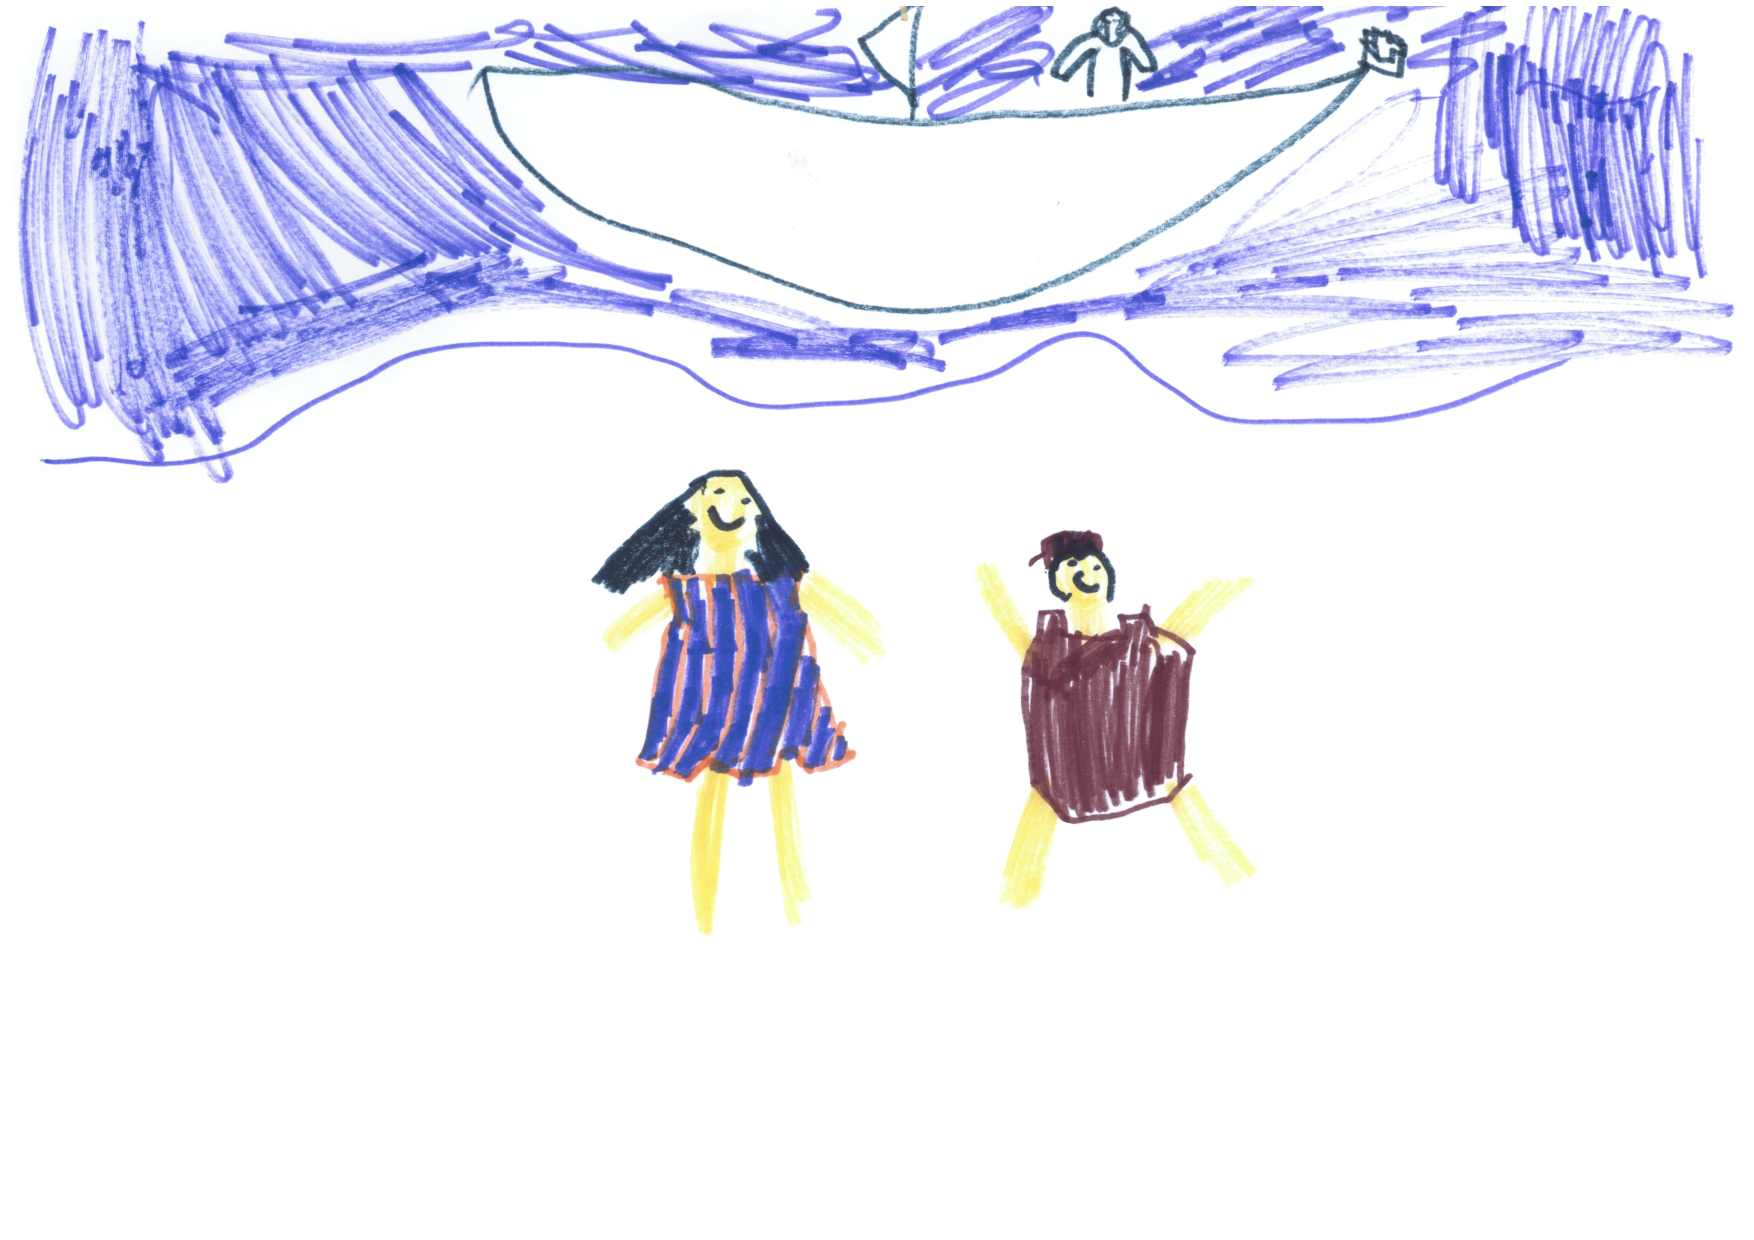
\includegraphics[width=.7\textwidth]{bilder/pirat1.pdf}
\end{figure}

Winnimon blickte fragend. Sie holte tief Luft und sagte: \enquote{Ich kann nicht fluchen. Mir fällt einfach kein Fluch ein. Du musst mir den besten Fluch verraten, den du kennst!}

\enquote{Aber warum willst du denn fluchen können?} Winnimon blickte fragend. \enquote{Du willst doch nicht etwa\dots?}

\enquote{Aber natürlich will ich auch Piratin werden! Meinst du ich will mein ganzes Leben hier verbringen? Ich will auch raus und die Welt sehen. Und jetzt hab ich dir geholfen, jetzt musst du mir helfen!}

Winnimon sah das sofort ein. Ihm ging es ja genauso. Und er zögerte nicht lange und verriet Drude seinen Lieblingsfluch. Das war er ihr schuldig, da gab es keine Frage. Ihm würde schon etwas einfallen.

Als beide zurück im Dorf waren, merkten sie gleich, dass etwas nicht stimmt. Vorbei am Haus von Winnimon sahen sie es auch schon. Ihm Hafen waren riesige Segel zu sehen und ganz oben auf dem höchsten Masten wehte die schwarze Fahne mit dem Totenkopf. Die Piraten waren da!

Sofort liefen die beiden hinunter zum Hafen. Das ganze Dorf hatte sich schon versammelt. Ein dicker Pirat stand in der Mitte der Menschenmenge auf einem Fass und rief:

\enquote{Liebe Leute. Mein Name ist Francisco San. Ich diene unter Barnabas Rotwild als erster Leutnant auf der Drachenblume, dem grössten Piratenschiff weit und breit. Wir sind gekommen, um zu fragen, ob jemand hier an Bord anheuern will. Wir nehmen zwei Schiffsjungen auf. Kommt mit uns, lernt die Welt kennen und werdet reich oder geht mit uns unter. Ihr alle kennt die drei Prüfungen. Aus all denen, die sie bestehen, nehmen wir zwei von euch auf. Freiwillige, tretet vor! Lang leben die Piraten!}

Alle Jungen und Mädchen waren sofort sehr aufgeregt, alle wollten mit. Nachdem sich die ersten getraut hatten vorzutreten, gaben sich auch Winnimon und Drude einen Ruck und stellten sich neben die anderen, alle in eine Reihe. Das alles so schnell gehen würde, hätten sie ja nie gedacht.

\enquote{Na dann wollen wir mal sehen.} Leutnant Francisco San schritt langsam die Reihe der Jugendlichen ab und zwirbelte dabei seinen Bart. \enquote{Ihr nehmt euch jetzt alle einen Stift und ein Stück Papier von dort drüben und schreibt folgende Wörter auf: Schatztruhe, Gewitter, arbeiten und Papagei.}

Die Prüfung war nur für zwei Jungen und ein Mädchen ein Problem, die ohne zu diskutieren den Stift hinlegten und aus der Reihe der Jugendlichen zurücktraten. Die waren schon durchgefallen. 

Bei der nächsten Prüfung, dem Fluchen, ging es sehr schnell zu. Jeder musste sich auf das Fass stellen und einmal so laut fluchen wie er konnte. 

\enquote{Dreibeiniger Hund}, \enquote{Vierauge}, \enquote{Vogelscheuche}, das waren so die Flüche die man hören konnte. Aber der Leutnant war nicht zufrieden. Die Flüche hätten alle schon einen längeren Bart als Kapitän Rotwild. Und wenn man so lange auf See ist und man immer die selben Flüche hört, wird einem echten Piraten sofort langweilig. Dann kamen Drude und Winnimon an die Reihe. Drude bestand den Test sofort mit mit dem {\it dreifach stinkenden Pups einer toten Ratte}. Sie war Winnimon sehr dankbar, denn mehr als Schwachkopf, aber da musste sie selbst zugeben, dass das sehr langweilig ist.

Winnimon brachte erst kein Wort heraus. So lange hatte er sich darauf verlassen, einen prima Fluch zu haben, dass er sich keinen neuen überlegt hatt. Wie angewurzrlt stand er auf dem Fass, aber dann brach es aus ihm heraus:

\enquote{Eitrige Warze am Bauch einer toten Ratte}. Der Leutnant lachte und sagte bestanden.

Danach waren nur noch drei Jugendliche im Rennen. Drude, Winnimon und ein weiterer Junge. Einer von denen die immer über Winnimon gelacht hatte, wenn der versucht hatte zu schwimmen. Er fühlte sich deswegen auch schon siegessicher, sprang gleich ins Meer, schwamm ein paar Züge und kam mit triumphierenden Lachen wieder aus dem Wasser. Drude machte es ihm nach. Jetzt waren alle Augen auf Winnimon gerichtet. Der sprang aber nicht gleich ins Wasser, sondern kletterte erst auf das Schiff, stellte sich auf die Reeling und blickte nach unten. Das Wasser war jetzt doch viel weiter weg, als er gedacht hatte. 

Die anderen Jungen fingen schon an zu lachen, da sprang Winnimon im weiten Bogen und mit Kopf voran in die nächste Welle. Als er wieder hoch kam, hatte er zwar Wasser geschluckt, liess sich aber nichts anmerken und schwamm zurück an Land. Alle klatschten, damit hätte niemand gerechnet.

Nur der Leutnant war unzufrieden. \enquote{Wir wollten ja nur zwei mitnehmen.} sagte er. \enquote{Na gut, dann stelle ich jedem von euch eine Frage. Du}, und dabei zeigte er auf Winnimon, \enquote{Wie heisst unser Piratenschiff}.

\enquote{Drachenblume!} Das war leicht für Winnimon. Er hatte schon so oft von der berühmten Drachenblume reden hören, er wusste alles über dieses Schiff. 

\enquote{Und Du}, diemal zu dem Jungen gewand \enquote{Was für ein Schiffstyp ist die Drachenblume?} Der Junge wurde bleich und ganz verlegen. Er wusste es nicht.

\enquote{Eine Galeone} rief Drude. Na klar, Drude wusste eigentlich fast alles. Sie war die beste der Klasse gewesen. 

\enquote{Damit ist es entschieden!} rief der Leutnant. \enquote{Ihr beiden kommt mit! Und wie es der Piratenbrauch verlangt, geht ihr sofort an Bord. Ihr dürft euch nicht nochmals umdrehen und von niemandem verabschieden. Euer altes Leben ist vorbei, ihr seid jetzt Piraten an Bord der Drachenblume.}

Winnimon und Drude hatten Tränen in den Augen. Das war jetzt doch alles sehr schnell gegangen. Aber sie bleiben tapfer und drehten sich nicht nochmals um, als sie auf das Schiff gingen. Sie hörten nur wie die Dorfbewohner klatschten. Als sie das Schiff betraten, fingen die Piraten an, alte Piratenlieder zu singen.
\begin{verse}\it
15 Mann auf eines Toten Truh'\\
Johoho und ne Buddel voll Rum\\
Versoffen und beim Teufel ist die ganze Crew\\
Johoho und ne Buddel voll Rum\\
\end{verse}
\section*{\center $\skull$ Die ersten Tage als Pirat $\skull$}

Die Wellen brandeten unaufhörlich gegen die Drachenblume. Nicht eine Minute lag das Schiff ruhig im Wasser. Die letzten sind hart gewesen. Winnimon war seekrank geworden und musste sich die ganze Zeit übergeben. Jetzt ging es aber schon besser, jedenfalls dem Bauch. Der Smudje hatte die ganze Zeit neben ihm gesessen und das wildeste Seemannsgarn gesponnen. So sagt man, wenn Seeleute Geschichten erzählen, die gar nicht wirklich stimmen. Jedenfalls bildete sich Winnimon ein, dass die Geschichten wohl nicht stimmen können. Vor riesigen Kraken hatte der Smudje erzählt, die ganze Schiffe in die Tiefe reissen konnten. Und von schlimmen Piratenkapitänen, die noch nach ihrem Tod als Gespenster andere Schiffe überfielen. Von Sirenen, die so schöne Stimmen hatten, dass wenn man sie hört, unbedingt zu ihnen hinsegeln möchte, aber dann gegen ein Riff fährt und versinkt. So Geschichten eben. Dazu hatte der Smudje immer laut gelacht und sich Trockenfleisch mit seinem riesigen Messer abgeschnitten.

Die grosse Überraschung für Winnimon war, dass man doch mehr lernen musste, als er dachte. Das hätte er nicht gedacht. Er musste sich eine Liste mit den wichtigsten Begriffen machen, die er auswendig lernen musste. Das war schon notwendig, um den Smutje verstehen zu können, der sagte immer nur Sätze wie:

\enquote{Beim Klabautermann, versenk mich doch! Wenn ihr Sprotten nicht man bald die Klüsen zu macht, dann hol' ich euch ein Donnerbräu, dass ihr glaubt ich seh aus wie Jolly Roger!}

Umständlicherweise hatte alles im und am Schiff einen eigenwilligen Namen wie Besanmast, Sechspfünder, Kombüse und ähnlich unverständliches. Das musste gepaukt werden, da half alles nichts. Dazu kamen noch andere Dinge. Zum Beispiel, dass es unterschiedliche Piraten gab. Die Piraten der Drachennest waren Bukanier und als solche keine bösen Piraten. Sie überfielen eigentlich nur spanische Schiffe. Das Gold, dass sie dabei erbeuteten brachten sie zurück nach Südamerika, wo es die Spanier selbst den Inkas gestohlen hatten. Denen gaben sie ihr Gold zurück, natürlich aber erst nach Abzug eines grosszügigen Anteils.

Dann war noch zu lernen, wie man richtige Seemannsknoten machte, wie man schnell in den Ausguck, Krähennest genannt, klettern konnte, ohne dass es einem schwindelig wurde und vieles mehr.






Winnimon lag in seiner Hängematte im Achterdeck und wollte sich kurieren, als die Schiffsglocke geläutet wurde. Alle Mann an Deck, hiess das. Ein Sturm war aufgezogen, da wurden alle Hände gebraucht. Winnimon musste an Leinen ziehen und Taue tragen, hier etwas festbinden und dort etwas holen. Viele Stunden dauerte der Sturm. Er hatte gar keine Zeit, Angst zu haben. Die anderen Piraten machten nicht den Eindruck, als ob etwas Besonderes vor sich ging. Als der Sturm endlich vorbei war, und alle irgendwo an Deck sassen und sich ausruhten, stellte sich Kapitän Barnabas Rotwild stellte sich auf die Brücke und rief mit wuchtiger Stimme:

\enquote{Männer, Frauen. Ich danke euch für eure Arbeit während des kleinen Sturms.}

Von wegen klein, dachte Winnimon.

\enquote{Wie ihr wisst, haben wir zwei Landratten an Bord gehabt. Ich glaube, nach diesem Sturm sind sie echte Seeleute geworden!} Dabei blickte er lachend zu Winnimon und Drude.

\enquote{Jetzt müssen wir nur noch Piraten aus ihnen machen. In zwei Tagen erreichen wir die Insel Pingelap. Auf Pingelap liegt ein Schatz, dass weiss ich. Die beiden Neuen sollen sich ein Boot nehmen und den Schatz bergen. Dabei werden sie auf sich allein gestellt sein. Haben sie den Schatz, sind sie vollwertige Piraten. Haben sie ihn nicht, lassen wir sie nicht wieder an Bord.}

Winnimon war bleich geworden und Drude auch. Sie fassten sich an die Hand und flüsterten \enquote{Wir schaffen das!}







Winnimon klatschte mit einer Hand nach einer Fliege. 

\enquote{Harrr!} hörte er hinter sich den alten Smudje schnaufen. ``Das ist nicht gut, sage ich, wenn einer jemanden tötet, der schlauer ist als er selbst!''

Winnimon wusste erst gar nicht, was der Smutje meinte. Er hatte ja noch nie jemanden getötet. ``Die Fliege meine ich, Du Grünspan''

Und noch bevor Winnimon etwas erwedern konnte, erklärte der Smutje: ``Auch bei Fleigen gibt es Mann und Frau, sonst könnte es keine kleinen Fliegen geben. Kannst Du die unterscheiden?'' 

``Ähhm''

``Siehst Du, und Fliegen können das. Alle. Sie wissen also mehr als Du.''



\section*{\center $\skull$ Auf der Papageieninsel $\skull$}
Noch bevor die Sonne aufgegangen war, wurde Winnimon vom Smutje geweckt.

\enquote{Winnimon, aufwachen. Du gehst heute auf Schatzsuche.} Winnimon war wie elektrisiert. Noch ehe der Smutje sich einmal richtig umgedreht hatte, war Winnimon aus seiner Koje gesprungen und stand angezogen da.

\enquote{Leise, die anderen schlafen noch. Hier ist ein Sack mit deinem Proviant. Du nimmst jetzt das Beiboot und ruderst zu der kleinen Insel da vorne. Auf der Insel ist ein Berg und in dem Berg eine Höhle und in der Höhle der Schatz- Du gehst voraus und suchst den Schatz, wir anderen kommen später hinterher und helfen dir beim Transport. Das ist auch nicht weiter gefährlich, die Insel ist unbewohnt und gefährliche Tiere gibt es auch nicht.}

So ruderte Winnimon durch die Dunkelheit, immer ein Schlag nach dem anderen. Nach einer Stunde war bei der Insel, die Sonne war mittlerweile auch aufgegangen und wärmte schon recht angenehm. Also nochmals schnell ins Meer gesprungen, denn Weg zu dem Berg sah lang aus und der Berg war hoch. 

Gerade als Winnimon wieder mit dem Kopf aus dem Wasser guckte hörte er eine krächzende Stimme.

\enquote{Besuch, Besuch, Besuch, wir haben Besuch.} und sofort wiederholte ein grosser Chor von genauso krächzenden Stimmen \enquote{Besuch, Besuch, Besuch, Besuch.}

Winnimon verhielt sich ganz still und sah sich um. Kein Mensch war zu sehen, lediglich ein paar bunte Vögel sassen auf den Bäumen. Wo waren die vielen Menschen versteckt, die da gerade noch gerufen hatten. Vorsichtig kam Winnimon aus dem Wasser und schlüpfte in seine Kleider.

\enquote{Was will er wohl? Was will er wohl?} hörte er die Stimmen wieder. Er nahm seinen Mut zusammen und rief laut: \enquote{Ich bin Winnimon, Pirat auf der Drachenblume. Wer seid ihr? Zeigt euch ihr Feiglinge!}

Und der Chor antwortete: \enquote{Er sieht uns nicht, er sieht uns nicht.}

Da begriff Winnimon, wer da gerufen hatte. Die Papageien! Natürlich, davon hatte er gehört, dass Papageien sprechen können. Da kam ihm eine Idee. Er öffnete den Sack mit dem Brot, den er vom Smutje bekommen hatte, brach etwas Brot ab und verstreute es am Strand. Dann setzte er sich daneben und wartete. Es dauerte auch nicht lange, da kamen die ersten Papageien angeflogen. Herrlich bunt glitzerten ihre Federn in der Morgensonne. Winnimon war in diesem Augenblick sehr zufrieden mit sich und seinem Leben.

Der erste mutige Papagei landete ganz in seiner Nähe. Er neigte den Kopf zur Seite und kam langsam immer näher gehüpft. Er schnappte sich ein Stück vom Brot und sprang wieder zurück. Von dem Beispiel ermutigt kamen noch mehr Papageien und knabberten Brot. 

\enquote{Ich bin hier, weil ich einen Schatz suche}, begann Winnimon zu sprechen. 

\enquote{Einen Schatz sucht er, einen Schatz.} Winnimon begann es etwas zu nerven, dass die papageien immer alles doppelt sagen mussten.

\enquote{Aber wir verraten nicht, wo leckersten Früchte wachsen, verraten wir nicht.} Winnimon musste lachen. Papageien halten natürlich ganz andere Dinge für einen Schatz als Menschen.

\enquote{Nein, ich will euch nicht eure Früchte wegnehmen. Ich suche einen Schatz aus Gold und Edelsteinen. Er muss in einer Höhle in einem Berg sein.}

Nachdem Winnimon versprechen musste, dass er tatsächlich keine Früchte wollte, willigten die Papageien ein, ihm den Weg zu zeigen. Sie flogen voraus und Winnimon immer hinterher. Erst fand er es lustig, dass die Papageien immer ein lustiges Lied zu singen wussten, aber irgendwann bekam er von den krächzenden Stimmen Kopfschmerzen. Aber es wäre natürlich sehr unhöflich gewesen, die Vögel zu bitten aufzuhören. Gegen Mittag erreichten sie den Fuss eines Berges. Die Papageien begleiten ihn noch ein Stück, meinten aber dass Papageien niemals auf Berge fleigen würden und dass er ab hier alleine weiter müsse. Aber er müsse immer nur in Richtung Bergspitze weiter, dann käme er an die Höhle und in der Höhle müsse der Schatz sein, sie hätten das jedenfalls so von den Adlern gehört, die hier lebten. Zum Abschied bekam er noch eine besonders schöne rote Feder geschenkt, die er sich an den Hut stecken konnte.

Der Aufstieg war zwar anstrengend, machte aber vor allem auch Spass. Winnimon kletterte nämlich sehr gerne. So dauerte es auch nicht lange, bis er tatsächlich den Eingang einer Höhle gefunden hatte. Er ging hinein und wartete, bis sich seine Augen an die Dunkelheit gewöhnt hatten.

Überall hingen Spinnweben an den Wänden und an der Decke schliefen Fledermäuse, Kopf nach unten, wie die das so machen. Ein bisschen unheimlich war Winnimon jetzt schon zu Mute. Aber als Pirat hat man keine Angst zu haben, das gehört zur Berufsehre dazu. Also ging Winnimon immer tiefer und tiefer in die Höhle, bis er plötzlich ein Schnarchen hörte. 

Winnimon hielt die Luft an, um sich bloss nicht durch das kleinste Geräusch zu verraten. Langsam ging er weiter nach vorne. Er musste erst ein grosses Spinnennetz, das vom Boden bis zur Decke der Höhle reichte kaputt machen, um zu sehen, wer da so schnarchte. Zwei Dinge konnte Winnimon im Halbdunkel erkennen: die Schatztruhe, aber auch einen riesigen Höhlenbär, der es sich ausgerechnet auf der Truhe gemütlich gemacht hatte.

Und dann noch etwas drittes. Die Spinne, deren Netz er gerade kaputt gemacht hatte, sass auf seinem Arm und krabbelte an ihm hoch. Das Tier war mindestens so gross wie die Hand des Smutje und sie hatte Haare am ganzen Körper. Winnimon musste allen Mut zusammen nehmen, um nicht laut zu schreien und den Bären zu wecken.

Die Spinne krabbelte imemr höher und höher. Winnimon hatte vor Angst Schweissperlen auf der Stirn. Was, wenn die Spinne gifitg war? Sollte er sie versuchen abzuwischen? Dann würde die vielleicht denken, er will sie angreifen und biss zu. Also bliess er die Spinne so kräftig an wie er konnte. Die hielt an und liess sich an einem Faden zu Boden und lief davon.

Winnimon fühlte sich, als hätte er seit Stunden einen schweren Rucksack tragen müssen und diesen jetzt absetzen können, so erleichtert war er. Aber was sollte er jetzt mit dem Bären machen? Da kam er auf eine List. Er setzte seinen Hut ab und band eine lange Schnur daran. Das andere Ende der Schnur knüpfte er an einen grossen Stein, der draussen vor der höhle direkt am Abhang des Berges lag.

Zurück beim Bären nahm Winnimon die Feder, kitzelte den schlafenden Bären an der Nase und legte ihm den Hut direkt auf das gesicht, so dass er erst nichts sehen konnte.

Der Bär erwachte, merkte dass ihm etwas im Gesicht und fing an zu brüllen und nach dem frechen Hut mit der tatze zu schlagen. Diesen Augenblick nutze Winnimon um aus der Höhle zu rennen und gegen den Stein mit der Schnur zu treten. Sich selbst versteckte er neben dem Eingang der Höhle. Der Stein fing an den Berg hinab zu kullern und riss den Hut hinter sich her. Der Bär jagte dem Hut nach rannte aus der Höhle und den Abhang hinab. unten angekommen, merkte er, dass der Hut wohl keine Gefahr war. Er reckte sich noch halb verschlafen und wo er einmal munter war, konnte er gleich twas zu fressen suchen.

Winnimons Plan war aufgegangen. Der Bär war weg. Mit ganzer Kraft zog er die Kiste aus der Höhle, setzte sich oben darauf und sauste mit ihr den Berg hinab, bis fast zum Strand. Die anderen Piraten waren inzwischen auch gelandet und ärgerten sich mit den Papageien herum, die sofort angefangen hatten die Piraten wüst zu beschimpfen und diese schimpften zurück, wie es eben auch zur Piratenehre gehört. So hatten sie scheinbar schon den ganzen morgen zusammen gezankt, als Winnimon eintraf.

Als sie sahen, dass Winnimon den Schatz sogar schon geholt hatte, brachen alle in Jubel aus. Und dann lernte Winnimon den nächsten Piratenbrauch kennen, der sofort zu seinem Lieblingsbrauch wurde. Wenn ein Schatz geborgen wurde, wird ein Fest gefeiert. Aber das richtig. Ein grosses feuer wurde angezündet und die leckersten Sachen gebraten. Die Papageien waren auch nicht kleinlich und bekamen als Austausch gegen Brot die saftigsten Früchte der Insel. Lieder wurden gesungen, wobei Winnimon feststellte, dass die Piraten die noch scheusslicheren Stimmen haben, als Papageien, aber das macht ja eigentlich nichts. Hauptsache, alle hatten Spass.


\section*{\center $\skull$ Der Schatz $\skull$}
Am nächsten Morgen, na ja, eigentlich war es schon mittags, bis die letzten Piraten aus ihren Sandgruben, die sie sich als bett gegarben hatten, aufgestanden waren. Winnimon war als erster munter gewesen und sich mit den Papageien unterhalte. Der Smutje brummelte etwas wie: 

\enquote{Wenn Du auch irgendwann mal Rum trinken darfst, wirst du morgens auch nicht mehr der erste sein, der wach ist.} Was immer das bedeuten sollte.

Die Piraten versammelten sich feierlich um die Truhe und der Smutje nahm sein Schwert und hebelte die Truhe auf. Und tatsächlich. Die Kiste war voll gefüllt mit Gold und Edelsteinen. Kelche aus purem Gold waren dabei, kostbarster Schmuck und sogar eine goldene Krone. Alle Piraten schwiegen erst ehrfürchtig, dann fingen alle an zu jubeln.

Der Kapitän streichte sich mit der Hand durch seinen langen Bart und rief:

\enquote{Freund, Piraten. Einen herrlichen Schatz haben wir hier geborgen! Ich glaube, dass dies unsere letzte Fahrt als Piraten gewesen ist, denn jetzt sind wir reich. Wir können zu unseren Familien zurückkehren!}

Erneut jubelte die versammelte Mannschaft. Sicher waren alle gerne Piraten, aber wirklich freiwillig war das niemand. Viele hatten Familien, die sie nur sehr selten sahen, manchmal nur einmal im Jahr. Piraten waren sie alle nur, um Geld zu verdienen. Und davon hatten sie jetzt genug.

\enquote{Wie es Brauch ist}, fuhr der Kapitän fort, \enquote{Darf ich mir als erstes meinen Anteil nehmen und mir etwas aussuchen. Aber diesen Schatz verdanken wir Winnimon. Er soll heute als erster wählen dürfen!} 

Und ein drittes Mal jubelten alle, diesmal aus Zustimmung. Winnimon war verlegen geworden, aber der Smutje schubste ihn einfach sanft zu der Truhe. Winnimon wisste gar nicht, was er nehmen sollte und war ganz rot im Gesicht geworden. Der Smutje lachte und sagte:

\enquote{Du bist der König dieses Schatzes, also sollst du die Krone bekommen.} Mit diesen Worten setzte er Winnimon die Krone auf. Dann waren der Reihe nach die anderen Piraten dran, jeder durfte sich etwas nehmen.

Am Abend, als sie wieder auf dem Schiff waren, nahm der Smutje Winnimon zur Seite und sprach:

\enquote{Ich werde mir von meinem Anteil ein kleines Lokal irgendwo am Meer kaufen. Ich habe mich auf dem letzten Landgang in eine Frau auf Madagaskar verliebt, da werde ich hinfahren und fragen, ob sie mit mir zusammen ein Restaurant eröffnen will. Wir werden Fische braten und an Seeleute verkaufen. Und du, was hast du vor?}

Das hatte sich Winnimon noch gar nicht überlegt. Was sollte er schon tun? Wo sollte er hin? zurück in das Dorf wollte er nicht mehr. 

\enquote{Ich werde Seemann bleiben. Ich will die Welt bereisen. Sehen, wie andere Menschen leben. Ich will Eisberge im Wasser sehen und Vulkane die Feuer ausspucken. Auf einem Kamel durch die Wüste reiten und auf die höchsten Berge klettern.}

Der Smutje freute sich. Das klang doch für einen Burschen im Alter von Winnimon nach einem guten Plan.

\enquote{Dann zeig mal deine Krone her. Wollen doch mal sehen, wie viel die Wert ist. Wenn sie wertvoll genug ist, kannst du deine Reisen als Passagier machen und musst nicht selber schuften.}

Winnimon wickelte die Krone aus dem Tuch, dass er zum Schutz um sie geschlungen hatte. Der Smutje prüfte die Krone von allen Seiten. Dann stutzte er und stampfte mit dem Fuss auf den Boden. Das war so üblich, wenn man jemandem unter Deck Bescheid geben wollte, zu kommen. Dazu brüllte er:

\enquote{Yaotl, komm mal her!} und zu Winnimon gewand fuhr er fort: \enquote{Siehst du hier auf der Krone die Symbole? Das ist Atztekenschrift. Yaotl ist Atzteke, vielleicht kann er uns das vorlesen.}

Und Yaotl, den alle nur Chaotl nannten, weil er ständig alles vergass, konnte tatsächlich die Schrift entziffern. Er las vor.

\enquote{Ich bin die Krone von Cacama, König von Texcoco. Wer mich trägt, dem gehört das Land der Acolhua und ist mein rechtmässiger Erbe.}

Yaotl sprang auf und verbeugte sich tief vor Winnimon.

\enquote{Dann bist du jetzt mein rechtmässiger König} sagte er. Winnimon und der Smutje waren viel zu verblüfft, um irgendetwas zu sagen.

\enquote{Ich will gar kein König sein} antwortete er nach einiger Zeit, \enquote{Aber ich will deinem Volk diese Krone zurückbringen.}

Die Sache war schnell besprochen. Das Land der Azteken lag ungefähr zwei Monate mit dem Schiff entfernt, was man damals als nicht so weit empfand. Der Plan war, Winnimon dort auszusetzen, damit der Krone zurückbringen könne. Und so wurde es auch gemacht. In der Zwischenzeit lernte Winnimon die wichtigsten Wörter auf Nahuatl, der Sprache der Acolhua.




  \hfill {\color{red}\decofourleft}
